\documentclass[english,version-2020-11]{uzl-thesis}


% Copy this file as a template for your thesis. You will have to take
% action at all places marked by
%
% !!!!!!!!!!!!!!!!!!!!!!!!!!!!!!!!!!
% !!! Your action is needed here !!!
% !!!!!!!!!!!!!!!!!!!!!!!!!!!!!!!!!!
%
% The first place your action is needed is the first line of this
% document:
%
%
% Language of the thesis:
%
% You must use either 'german' or 'english' above, depending on the
% language used in the main text. This will automatically setup a lot
% of things in the background.
%
%
% Version of the class:
%
% You must specify which version of the thesis class is to be
% used. This is important in case the class style changes in later
% years, but we still want an older thesis to look the same, even when
% things are changed in the class.
%
% Do not change or remove the version-xxxx key.
%
%
% Text encoding:
%
% Your thesis *must* be encoded in utf8 (unicode), which is the
% default in most editors these days. Do *not* change this to latin8.



%%%
%
% Main setup:
%
%%%
%
% You must use the \UzLThesisSetup command to specify numerous things
% about your thesis. This includes the entries on the title page, the 
% abstracts, and the bibliography style. You do so by specifying
% so-called "values" for so-called "keys". For instance, 
% for the key "Autor" you must provide your name as the value. You do
% so by writing 'Autor = {Max Mustermann}', that is, the value is put
% into curly braces. You can use the \UzLThesisSetup command
% repeatedly and the order in which you provide the keys is not
% important. 
%
% Everything shown on the title page must be in German -- even
% if the thesis is written in English! Just insert German text for
% German keys and English text for English keys (like 'Abstract' needs
% English text, while 'Zusammenfassung' needs German text).

\UzLThesisSetup{
  %
  % !!!!!!!!!!!!!!!!!!!!!!!!!!!!!!!!!!
  % !!! Your action is needed here !!!
  % !!!!!!!!!!!!!!!!!!!!!!!!!!!!!!!!!!
  %
  % First, specify the institut or clinic at which the thesis was
  % written. You get the logo file from them (make sure it has the
  % correct size, namely the same as the example). If they do not have
  % a logo, the university's default logo is used.
  %
  % The 'verfasst' gets two arguments. Change the first to {an der}
  % for clinics, as in 'Verfasst = {an der}{Medizinischen Klinik I}'
  %
  Logo-Dateiname        = {uzl-thesis-logo-itcs.pdf},
  Verfasst              = {am}{Institut für Theoretische Informatik},
  %
  % The titles:
  %
  Titel auf Deutsch     = {
     Sichere Steganographie auf ML-Basierten Kanälen
  }, 
  Titel auf Englisch    = {
    Secure Steganography on ML-Based Channels
  },
  %
  % Author and supervisor:
  % 
  % Note that the 'Betreuer' or 'Betreuerin' is the supervisor, that
  % is, the professor who officially supervises the thesis. If there
  % is also an assistent of the professor who helped (typically a
  % lot), use 'Mit Unterstützung von' to thank that person. If the
  % thesis was mainly written 'externally' at some company or another
  % institute, point this out using 'Weitere Unterstützung'. 
  % 
  % For your own name, do *not* add things like "BSc" or "BSc
  % cand.". For the supervisor, you should normally include
  % "Prof. Dr." or "PD Dr." (ask your supervisor, what is
  % appropriate), but nothing more (so no
  % "Univ.-Prof. Dr. Dr. h.c. mult." unless your supervisor insists).  
  %
  Autor                 = {Jeremy Boy},
  Betreuer              = {Prof. Dr. Maciej Liśkiewicz},
  % 
  % Optional: Supporting persons and institutions. The text should be
  % in German, even for an English thesis.
  %
%  Mit Unterstützung von = {Harry Hilfreich},
  % 
  %   Weitere Unterstützung = {
  %     Die Arbeit ist im Rahmen einer Tätigkeit bei der Firma Muster GmbH
  %     entstanden.
  %   },
  %
  %
  % Your Degree Programm (Studiengang)
  %
  % Specify 'Bachelorarbeit' or 'Masterarbeit' and the degree
  % programme. Make sure the name of programme is correct and not
  % some abbreviation or some incorrect variant. For instance:
  % 'Medizinische Ingenierwissenschaft', but not 'MIW';
  % 'Medizinische Informatik', but not 'Medizin-Informatik';
  % 'Informatik', but not 'Informatik (SSE)'.
  %
  % Use German names for German programmes and English names for
  % English ones, so 'Infection Biology', not 'Infektionsbiologie'. 
  % For programmes that have a German bachelor and an English master,
  % use the German name for a bachelor thesis and the English name for
  % the master thesis.
  %
  Bachelorarbeit,
  Studiengang           = {IT-Sicherheit},
  %
  % Date on which the thesis is turned in German, formatted the
  % traditional German way:
  %
  Datum                 = {\today},
  %
  % The English abstract. You must always provide abstracts in German
  % and in English. 
  %
  Abstract              = {
    Governmental and commercial adversaries increasingly threaten the confidentiality of encrypted communication.
    Steganography alllows confidential communication even in environments where cryptography is actively prohibited.
    The Meteor Stegosystem extends classical steganographic primitives for the use on channels based on generative models, such as GPT-2.
    Here, the secret text is embedded in the model's sampling scheme.
    In this thesis, I perform a statistical analysis of Meteor's performance and compare it with the results presented in the original paper.
    Subsequently, I present and evaluate different strategies for embedding secret text.
    The strategies optimize the length of generated messages against reliability and computational ressources required to generate and decrypt stegotexts.
    The strategies improve the reliability significantly while keeping achievable information density and required computational ressources justifiable.
  },
  Zusammenfassung       = {
    Staatliche und privatwirtschaftliche Akteure bedrohen zunehmend die Vertraulichkeit verschlüsselter Kommunikation.
    Steganographie ermöglicht vertrauliche Kommunikation auch dann, wenn die Nutzung klassischer Kryptographie verhindert wird.
    Das Meteor-Stegosystem erweitert klassische steganographischer Primitive für die Verwendung auf Kanälen, die auf generativen Modellen basieren, wie etwa GPT-2.
    Hierbei wird der Geheimtext in das Sampling des generativen Modells eingebettet.
    In dieser Thesis führe ich eine statistische Analyse der Performance des Meteor-Stegosystems durch und vergleiche diese mit den im Paper präsentierten Ergebnissen.
    Anschließend präsentiere und evaluiere ich unterschiedliche optimierte Strategien zur Einbettung des Geheimtexts.
    Die Strategien optimieren die Länge der erzeugten Nachrichten gegen Zuverlässigkeit und Berechnungsaufwand beim Erzeugen sowie Entschlüsseln von Stegotexten.
    Die Strategien verbessern die Zuverlässigkeit signifikant, während die erzielbare Informationsdichte und benötigter Rechenaufwand vertretbar bleiben.

  },
  %
  % Optional: 'Danksagungen' (German) or 'Acknowledgements'
  % (English). Both keys are optional and both have the same effect of
  % adding an acknowledgements text after the abstracts and before the
  % table of contents.
  %
  %Acknowledgements      = {
  %  This is the place where you can thank people and institutions, do
  %  not try to do this on the title page. The only exception is in
  %  case you wrote your thesis while working or staying at a company or abroad. Then you
  %  should use the \Latex{Weitere Unterstützung} key to provide a text
  %  (in German) that acknowledges the company or foreign
  %  institute. For instance, you could use texts like »Die Arbeit
  %    ist im Rahmen einer Tätigkeit bei der Firma Muster GmbH
  %    entstanden« or »Die Arbeit ist im Rahmen eines
  %    Forschungsaufenthalts beim Institut für Dieses und Jenes an der
  %    Universität Entenhausen entstanden«. Do not name and thank
  %    individual persons from the company or foreign institute on the
  %    title page, do that here. 
  %},
  % Bibliography style: Choose between
  % 
  % 'Alphabetische Bibliographie'
  % for all degree programmes in the natural sciences 
  % 
  % 'Numerische Bibliographie'
  % alternative for all other degree programmes
  % 
  % Either will load biblatex and setup the citation methods and the
  % bibliography styles correctly. You should not mess with them.
  % 
  Alphabetische Bibliographie,
  % Alternatively:
  % Numerische Bibliographie
}




%%%%%%%%%%%%%%%%%%%%
%
% Styling the thesis
%
%%%%%%%%%%%%%%%%%%%%
%
% Creating a visually pleasing layout and choosing fonts is not
% easy. Furthermore, different people have different preferences. Of
% course, for the University of Lübeck, the dean of studies could just
% force everyone to use one specific layout and font, but that seems a
% bit drastic and, also, it seems nice that thesis by different people
% have an individual style even though they all stick to the same
% overall structure.
%
% For these reasons, I (Till Tantau) have spend quite some time on
% designing a flexible layout and styling mechanism for theses.
%
% Basically, the overall structure of the thesis is fixed by the
% thesis class and so are many structural elements. For instance, you
% cannot change the order in which the abstract and table of contents
% are shown, you cannot move the bibliography elsewhere, indeed, the
% bibliography style is also fixed. Likewise, the text on the title
% page is fixed.
%
% Although many things are fixed, you *can* change several other
% things. For instance, you can change the font used for the main
% text, you can change which font is used for titles and headings or
% you can change whether titles and headlines are centered or flushed
% left.
%
% There are many LaTeX packages for changing such things. You are
% kindly asked *not to use them*. Rather, use (only) the options
% offered by the thesis class. All possible choices and combinations
% there have been tested by me and produce nice results; what happens
% with other packages no one knows and might no longer conform to what
% is expected by the university. As you will see, you still have a
% lot of options.
%
%
% Technical note: All styling is done via the command
%
% \UzLStyle{...}
%
% where ... is a key-value list just as for \UzLThesisSetup. The
% difference is just that everything having to do with styling as
% controlled by \UzLStyle, while the more “formal” setup keys are
% controlled by \UzLThesisSetup.
%
%%%
%
% Designs
%
%
% A \emph{design} is a whole set of font and layout options bundled
% together. They have been chosen in such a way that a visually
% pleasing “overall appearance” results.
%
%
% \UzLStyle{computer modern oldschool design}
%
% The look of this design mimics the “classical” way a paper or report
% created with \LaTeX\ looks like: The Computer Modern font is used,
% bold face fonts are used for headlines, only black and white are
% used as colors. This design reminds me of older scientific
% documents, especially from the computer science community where
% \LaTeX\ was used very early.
%
%
% \UzLStyle{computer modern basic design}
%
% A slightly less “oldschool” version of the previous design. It is
% still a classic design in the sense that it uses the Computer Modern
% font and that it still has this “good old \LaTeX” look, but some
% more modern aspects (like colors!) have been added.
%
% Note that this design uses Myriad for the title page (one of the
% “modern aspect”), which means that his font must be installed.
%
%
% \UzLStyle{computer modern scholary design}
%
% In my opinion, this is the ultimate “scholary design”: The thesis
% will look like it has been typeset by hand some 150 years ago and
% then printed by a university press. There is really nothing “modern”
% about it and the word in the name of the design is just part of the
% name of the “Computer Modern” font.
%
%
% \UzLStyle{pagella basic design}
%
% A, well, basic design that uses the Pagella font rather than the
% Computer Modern font. Especially the bold face version of this font
% looks nicer than the Computer Modern counterpart. Also, Pagella,
% while still having a “bookish” look, still feels a bit fresher than
% Computer Modern. 
%
%
% \UzLStyle{pagella centered design}
%
% A variant of the basic Pagella design that centers all
% headlines. A nice alternative to the basic version.
%
%
% \UzLStyle{pagella contrast design}
%
% This design tries to create some visual friction by contrasting the
% sans serif headline font (in bold!) with the main text. I find it a
% visually very interesting combination.
%
%
% \UzLStyle{alegrya basic design}
%
% The third variant of the basic design, this time using the Alegrya
% font. 
%
%
% \UzLStyle{alegrya scholary design}
%
% The Alegrya version of the previous “scholary” design. Unlike the
% Computer Modern version, this design does not look old, but more
% fresh -- while still creating the impression that the text must be
% about a very scientific subject. 
%
%
% \UzLStyle{alegrya stylish design}
%
% The design is quite similar to the scholary version for the Alegrya
% font, but with even more modern additions. “Stylish” is the word
% that comes to my mind.
%
%
\UzLStyle{alegrya modern design}
%
% A design that uses the sans serif version of the Alegrya font for
% the headlines. This is a nice modern overall design.
%
%%%




%%%%%%%%
%
% Now, include the package you need here using \usepackage. 
%
% However, many standard packages are already loaded by the class:
%
% amsmath, amssymb, amsthm, babel, biblatex, csquotes, etoolbox,
% filecontents, fontspec, geometry, hyperref, tikz (with libraries
% arrows.meta, positioning and shapes), varioref, url 
%
% Indeed, in many cases you will not need any extra packages.
%
%%%%%%%

\usepackage[inline]{enumitem}
\usepackage{todonotes}





\begin{document}

%
% The title page and table of contents will be inserted automatically
% here. 
%

% In a German thesis write: \chapter{Einleitung}


% !!!!!!!!!!!!!!!!!!!!!!!!!!!!!!!!!!
% !!! Your action is needed here !!!
% !!!!!!!!!!!!!!!!!!!!!!!!!!!!!!!!!!
%
% Replace with your own introduction:

\chapter{Introduction}

When governmental and private-sector adversaries try to breach the confidentiality of private communication, civil society requires means to defend their privacy.
Especially in authoritorian states, law enforcement continuously attempts to break or prohibit effective means of cryptography, especially when used for censorship-resistant communication.

\section{Motivation}

TODO

\section{Structure Of This Thesis}

Chapter 2 discusses previous works.
First, we will discuss steganography and provably secure steganography, introduced in \cite{Hopper04}.
Afterwards, we discuss how generative neural networks (GNNs) such as GPT-2 produce high-quality text iteratively.
Concluding, I will present the Meteor stegosystem, a provably secure steganographic system over ML-based channels as introduced by XYZ.

Chapter 3 provides an analysis of the correctness of the Meteor stegosystem. 
We will see that the Meteor stegosystem is not correct because of the way tokenization in GNNs work.
Afterwards, I will present algorithms which ensure correctness of Meteor on the receiver site.
Unfortunately, these algorithms pose overhead exponential in the length of the generated stegotext.

In chapter 4, I present a small modification to the Meteor stegosystem which allows two-way communication.
There, we embed a fixed amount of bits in each message, using the DialoGPT model developed by Microsoft \cite{Zhang20} to generate dialog-like messages.
This modification makes sure that the algorithms from chapter 3 can be applied more conveniently, since the exponential overhead is negligible for shorter messages.

In chapter 5, we will perform a security analysis of the Meteor stegosystem using Hopper's definition of secure stegosystem.
We will compare the definition of security used by the Meteor authors with the definition of security by Hopper.
We then will show that the Meteor stegosystem is not universally secure in Hopper's definition.

Finally, in chapter 6, I will discuss the results in a conclusion and give ideas for further research.

\chapter{Previous Work}

\section{Provably Secure Steganography}

Steganography extends the concepts of cryptography to hide the mere existence of a message.
This makes it robust against censorship and prohibition.
While cryptography can be used to hide the contents of a confidential message, its use is easily discoverable by adversaries.
Steganography is usually modelled using the Prisoner's Problem, as introduced by \cite{Simmons83}.
There, two prisoners Alice and Bob are imprisoned.
While they can exchange messages, their contents are surveilled by a Warden.
Alice and Bob now want to craft and exchange escape plans.
Warden observes messages exchanged between Alice and Bob.
He tries to distinguish the exchange of the escape plan from innocous messages.

In steganography, a message is represented by a sequence of documents from an underlying distribution.
Most approaches to steganography use photographs as underlying distribution and hide information in the images' noise.
If the original photograph is unknown to Warden, Alice can encode hidden text in the original photograph

In his doctoral thesis ``Toward a theory of Steganography'', \cite{Hopper04} establishes a cryptographic point of view on steganography. 
This allows us to do cryptanalysis on steganographic protocols.
In section 3, he defines a stegosystem as follows:

\begin{definition}
(Stegosystem, Hopper) A \emph{steganographic protocol} $\mathcal{S}$, or \emph{stegosystem}, is a pair of probabilistic algorithms:

\begin{itemize}
	\item $\mathcal{S}$.Encode (abbreviated $SE$) takes as input a key $K \in \{0,1\}*$, a string $m \in \{0,1\}*$ (the hiddentext), and a message history $h$.
		SE(K, m, h) returns a sequence of documents $s_1||s_2||\dots||s_l$ (the stegotext) from the support of $\mathcal{C})h^l$.
	\item $\mathcal{S}$.Decode (abbreviated $SD$) takes as input a key $K$, a sequence of documents $s_1||s_2||\dots||s_l$, and a message history $h$.
		SD(K, s, h) returns a hiddentext $m \in \{0,1\}*$
\end{itemize}
\end{definition}

We want our stegosystem to be correct.
To achieve that, the decoding of a given stegotext $s$, given the correct key $k$ and history $h$, should yield the original hiddentext $m$.
Hopper defines the correctness of a stegosystem as follows:

\begin{definition}
(Correctness, Hopper) A stegosystem $\mathcal{S}$ is \emph{correct} if for every polynomial $p(k)$, there exists a negligible function $\mu(k)$ such that $SE$ and $SD$ also satisfy the relationship:

$$\forall m \in \{0,1\}^{p(k)}, h \in D^* \colon Pr(SD(K, SE(K, m, h), h) = m) \geq 1 - \mu(k)$$

where the randomization is over the key $K$ and any coin tosses of $SE$, $SD$, and the oracles accessed by $SE$, $SD$.
\end{definition}

The introduction of a \emph{negligible} polynomial $\mu(k)$ allows the stegosystem to sometimes yield wrong results, but only with probability negligible in the length $m$.
While stegosystem with $\mu(k) = 0$ can exist, the introduction of negligible polynomials proves helpful for reductions on established cryptographic primitives. 

Since we want our stegosystem to be prone to analysis by warden, we also need a definition of security.
We want any warden to not be able to efficiently decode our stegotext $s$ to the original message $m$ without knowledge of our secret key $k$.
As described above in the Prisoners' Game, we don't want any warden to be able to distinguish a stegotext $s := SE(K, m, h)$ from a covertext $c$ randomly sampled from the underlying distribution $\mathcal{C}$.
If the warden is allowed to choose the hiddentext $m$ used to generate $s$, we call warden a \emph{chosen hiddentext attacker}. 

If the warden can distinguish the stegotext from a covertext, they have an advantage against the stegosystem in the distingushing game.
The insecurity of a stegosystem is the maximum possible advantage any attacker can have.
The attackers are limited by running time $t(k)$, number of queries $q(k)$ and total length $l(k)$ of hiddentexts.
Formally, Hopper defined a chosen hiddentext attack as follows:

\begin{definition}
(Chosen Hiddentext Attack, Hopper) In a chosen hiddentext attack, $W$ is given access to a ``mystery oracle'' $M$ which is chosen from one of the following distributions:

\begin{enumerate}
\item $ST$: The oracle $ST$ has a uniformly chosen key $K \leftarrow U_k$ and responds to queries $(m, h)$ with a StegoText drawn from $SE(K, m, h)$.
\item $CT$: The oracle $CT$ has a uniformly chosen $K$ as well, and responds to queries $(m, h)$ with a CoverText of length $\mathcal{l} = |SE(K, m, h)|$ drawn from $\mathcal{C}_h^{\mathcal{l}}$
\end{enumerate}

$W^M(1^k)$ outputs a bit which represents its guess about the type of $M$.

We define $W$'s advantage against a stegosystem $\mathcal{S}$ for channel $\mathcal{C}$ by

$$Adv_{\mathcal{S}, \mathcal{C}, W}^{ss}(k) = |Pr[W^{ST}(1^k)=1] - Pr[W^{CT}(1^k)=1]|$$

where the probability is taken over the randomness of $ST$, $CT$, and $W$. 

Define the insecurity of $\mathcal{S}$ with respect to channel $\mathcal{C}$ by

$$InSec_{\mathcal{S}, \mathcal{C}}^{ss}(t, q, l, k) = \max_{W \in \mathcal{W}}(t, q, l) \left\{ Adv_{\mathcal{S}, \mathcal{C}, W}^{ss}(k) \right\}$$

where $\mathcal{W}(t, q, l)$ denotes the set of all adversaries which make at most $q(k)$ queries totaling at most $l(k)$ bits (of hiddentext) and running in time at most $t(k)$.
\end{definition}

\section{Generative Neural Networks}

Generative Neural Networks (GNN) establish a model which approximate realistic distributions such as natural language.
In the last few years, the artificial intelligence community achieved tremendous progress in building powerful machine learning based models.
The Generative Pretrained Transformer 2 (GPT-2) by OpenAPI is one of the industry-standard approaches to (not only) text generation.
GPT-2 has been introduced in \cite{OpenAI19}.
This model works on a set of tokens, which are words or sub-words of the approximated distribution.
To generate a sentence, i.e. a sequence of tokens, the model requires a history as input and outputs a probability distribution for the next token, see \ref{fig-generative-network}.

On a high level, we can understand the ML model as a black box.
When given a history, the ML model first generates a logits vector for tokens $t_i$, more formally a list of 2-tuples $((z_1, t_1), (z_2, t_2), \dots, (z_n, t_n)),~ z_i \in ( -\infty, \infty )$.
In the next step, we convert the logits vector $z := (z_i)^{1 \leq i \leq n}$ to a probability distribution $(p_i)^{1 \leq i \leq n}$ with $\sum_{i=1}^n p_i = 1$ using the softmax function $\sigma$:

$$\sigma \colon \mathbb{R}^n \rightarrow (0,1)^n,$$
$$\sigma(z) = \left(\frac{e^{z_i}}{\sum_{j=1}^n e^{z_j}}\right)^{1 \leq i \leq n}$$

When combined, we get the black box for our ML model in \ref{fig-generative-network}.

\begin{figure}[htpb]
	\centering
	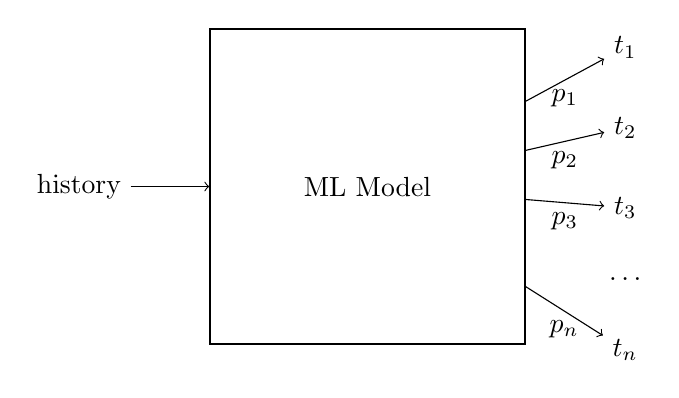
\begin{tikzpicture}
            \node[rectangle, draw=black, minimum width=4cm, minimum height=4cm] (oracle) {ML Model};
            \node[left=of oracle] (history) {history};
            \node[above right=-5mm and 1cm of oracle] (t1) {$t_1$};
            \node[below=5mm of t1] (t2) {$t_2$};
            \node[below=5mm of t2] (t3) {$t_3$};
            \node[below=5mm of t3] (t4) {$\dots$};
            \node[below=5mm of t4] (tn) {$t_n$};
            \draw[->] (history) -- (oracle);
            \draw[->] (oracle) -- node[midway,below] {$p_1$} (t1);
            \draw[->] (oracle) -- node[midway,below] {$p_2$} (t2);
            \draw[->] (oracle) -- node[midway,below] {$p_3$} (t3);
            %\draw[->] (oracle) -- (t4);
            \draw[->] (oracle) -- node[midway,below] {$p_n$} (tn);
	\end{tikzpicture} \label{fig-generative-network}
	\caption{Generative ML Model as black box function, taking a history as input.}
\end{figure}
To generate the next token in the sequence, there are basically two approaches:
\begin{enumerate*}[label=(\roman*)] \item \label{enum-gnn-most-likely} selecting the most likely token from the distribution or \item \label{enum-gnn-sample} sampling according to the generated distribution \end{enumerate*}.
While \ref{enum-gnn-most-likely} creates deterministic output, the generated sequences tend to be repetitive.
On the other hand, approach \ref{enum-gnn-sample} is not deterministic, but usually creates higher quality output.
For a comparison of GNN model outputs, see examples \ref{ex-gpt2-output} and \ref{ex-gpt2-output-sample}.

To use GPT-2 with the Python programming language, we can utilize the Huggingface Transformers library together with PyTorch.
In the most simple form, the pipeline API generates texts using not only GPT-2 but many other text generation models.
A Python program which generates the outputs in \ref{ex-gpt2-output} and \ref{ex-gpt2-output-sample} can be found at \ref{code-gpt2-demo}.

\lstinputlisting[language=Python, caption={Python program which generates text using the Huggingface Transformers Pipeline API}, label={code-gpt2-demo}]{code/pipeline_gpt2.py}


While the use of the pipeline API is very convenient to develop simple text generation or question answering programs, it abstracts some steps that we will need to intercept to use in a stegosystem.
A more sophisticated way to generate text using GPT-2 can be found in \ref{code-gpt2-logits-demo}.
The output of \ref{code-gpt2-logits-demo} resembles those shown in \ref{ex-gpt2-output-sample}. 
This code example shows how we can:

\begin{itemize}
	\item use a tokenizer to convert strings to a vector of tokens
	\item use the model to get a logits vector
	\item transform the logits vector into a probability distribution using the softmax function
	\item sample the next token from the distribution
	\item convert a vector of tokens to a string using the tokenizer
\end{itemize}


\lstinputlisting[language=Python, caption={Python program which generates text using the Huggingface Transformers}, label={code-gpt2-logits-demo}]{code/logits_demo_gpt2.py}



\begin{example}[Example of GPT-2 model output without sampling]
	Hello, I'm a language model, not a programming language. I'm a language model. I'm a language model. I'm a language model. I'm a language model. I'm a language model.
	\label{ex-gpt2-output}
\end{example}

\begin{example}[Example of GPT-2 model output with sampling]
	Hello, I'm a language model, I'm a problem solver in languages."

	At the same time, she said we can understand an idea like "reactive programming," because programming is what you create
	\label{ex-gpt2-output-sample}
\end{example}

\section{Meteor Stegosystem}

TODO 

\chapter{Correctness}

TODO

\section{Ambiguous Tokenization}

TODO

\chapter{Two-Way-Communication}

TODO

\chapter{Security Analysis}

TODO

\section{Comparison Of Meteor's And Hopper's Security Game}

TODO

\chapter{Conclusion}


% In a German thesis write: \subsection{Zusammenfassung und Ausblick}


% !!!!!!!!!!!!!!!!!!!!!!!!!!!!!!!!!!
% !!! Your action is needed here !!!
% !!!!!!!!!!!!!!!!!!!!!!!!!!!!!!!!!!
%
% Replace the following with your conclusion

TODO write a conclusion.

% Normally, the bibliography comes next at this point. Do *not* (try
% to) include further indices and tables like an index or
% a list of figures or a list of tables or such things. Nobody
% actually uses them and they just use up space. 
%
% You *can* however include a glossary, if this seems appropriate. It
% goes here as an unnumbered chapter. Most thesis will *not* need a
% glossary: a well-written text (re)explains strange words and
% concepts as necessary. However, there are situations where a
% glossary may be helpful.














%%%
% 
% Bibliographies
%
%%%
%
% The uzl-thesis class will load biblatex for the bibliography
% management. This is a powerful package, see its documentation for
% details. The styles will be setup correctly and automatically by
% choosing one of the two style keys as described earlier.
%
% In order for the bibliography to work, run latex in the following
% order (which is the standard order):
% 
% > lualatex thesis-example
% > bibtex thesis-example
%e > lualatex thesis-example
% 
% Add BibTeX files using \addbibresource or use the {bibtex entries}
% environment (see below).
%
%%%
%
% Although everyting is normally setup automatically, you can change
% the options passed to biblatex using the key 'biblatex';
% for instance,
%
%   \UzLThesisSetup{biblatex={firstinits=false}}
%
% will switch off shortened first names. Normally, you will not need
% this key in your preamble. 
% 
% Note that the bibtex program is used as the 'backend' of biblatex
% by default (rather than biber, which is the preferred program of
% biblatex). This means that you can (and must) run *bibtex* after you
% have run lualatex on your thesis. If you wish to use biber instead
% of bibtex, say 'biblatex={backend=biber}'. 
% 
%%%
%
% The following environment is optional. It allows you to keep the
% bibtex entries for your thesis right here in the thesis file. What
% happens is that each time this tex file is processed, the contents
% of the following environment gets written to the file
% \jobname-bibtex-entries.bib (this file gets overwritten each
% time). Independently, \addbibresource{\jobname-bibtex-entries.bib}
% is always called if the file \jobname-bibtex-entries.bib
% exists. 
%
% In result, you can edit and keep the bibliography's bibtex entries
% right here. If you change something here, run latex, then bibtex,
% then latex once more.
%
% If you would like to manage the bibtex entries in a separate file,
% remove the below environment, delete the \jobname-bibtex-entries.bib
% file and instead write
%
% \addbibresource{filename-of-your-bibtex-file.bib}
%
% in the preamble.
%
%%%


% !!!!!!!!!!!!!!!!!!!!!!!!!!!!!!!!!!
% !!! Your action is needed here !!!
% !!!!!!!!!!!!!!!!!!!!!!!!!!!!!!!!!!
%
% Replace following example entries with the ones of your thesis.

\begin{bibtex-entries}
@article{Simmons83,
   author={Simmons, Gustavus J.},
   title={The Prisoners' Problem And The Subliminal Channel},
   year=1983,
   pages={1-2}
}
@inproceedings{Hopper04,
  title={Toward a theory of Steganography},
  author={Manuel Blum and Nicholas Hopper},
  year={2004}
}
@inproceedings{Zhang20,
    title = "{DIALOGPT} : Large-Scale Generative Pre-training for Conversational Response Generation",
    author = "Zhang, Yizhe  and
      Sun, Siqi  and
      Galley, Michel  and
      Chen, Yen-Chun  and
      Brockett, Chris  and
      Gao, Xiang  and
      Gao, Jianfeng  and
      Liu, Jingjing  and
      Dolan, Bill",
    booktitle = "Proceedings of the 58th Annual Meeting of the Association for Computational Linguistics: System Demonstrations",
    month = jul,
    year = "2020",
    address = "Online",
    publisher = "Association for Computational Linguistics",
    url = "https://aclanthology.org/2020.acl-demos.30",
    doi = "10.18653/v1/2020.acl-demos.30",
    pages = "270--278",
    abstract = "We present a large, tunable neural conversational response generation model, DIALOGPT (dialogue generative pre-trained transformer). Trained on 147M conversation-like exchanges extracted from Reddit comment chains over a period spanning from 2005 through 2017, DialoGPT extends the Hugging Face PyTorch transformer to attain a performance close to human both in terms of automatic and human evaluation in single-turn dialogue settings. We show that conversational systems that leverage DialoGPT generate more relevant, contentful and context-consistent responses than strong baseline systems. The pre-trained model and training pipeline are publicly released to facilitate research into neural response generation and the development of more intelligent open-domain dialogue systems.",
}
@inproceedings{OpenAI19,
  title={Language Models are Unsupervised Multitask Learners},
  author={Alec Radford and Jeff Wu and Rewon Child and David Luan and Dario Amodei and Ilya Sutskever},
  year={2019}
}
\end{bibtex-entries}



% If you need to have an appendix (I advise against it), insert it
% here using, first, \appendix and then \chapter and then,
% possibly, \section. 
%
% \appendix
%
% \chapter{Technical Appendix}
%
% \section{Experimental Parameters} % possibly
%
% Again, I advise against using an appendix.


\end{document}

%  LocalWords:  LaTeX tex moretexcs Lübeck pdf uzl lualatex bibtex th
%  LocalWords:  TechReport Kernighan Lamport's Tantau's Tantau cls kZ
%  LocalWords:  Mustermann emacs oldschool pdflatex texmf utf biber
%  LocalWords:  biblatex Alphabetische Bibliographie Numerische VIIa
%  LocalWords:  varioref german Einleitung Beiträge dieser Arbeit xml
%  LocalWords:  Ergebnisse Verwandte Arbeiten Aufbau nucleotide VIIc
%  LocalWords:  ensembl amino phylogenetic Alexa Siri decrypt versa
%  LocalWords:  cryptographic pre nondeterministic deterministically
%  LocalWords:  Beutelspacher Untersuchungen zum genetischen sep llcc
%  LocalWords:  Beispiel tikz jpg png Alegrya Kasimir Malewitsch PGF
%  LocalWords:  Lamport Institut für Theoretische Informatik zu url
%  LocalWords:  Universität Springer DowneyF Downey Parameterized doi
%  LocalWords:  BibLaTeX Kime Philipp urldate Mittelbach hyperref Lua
%  LocalWords:  Rahtz Oberdiek Heiko Braams Bezos López fontspec Das
%  LocalWords:  Arseneau amsmath ist Tipps und zur Formulierung
%  LocalWords:  mathematischer Gedanken Mathematik Studienanfänger
%  LocalWords:  Albrecht Vieweg Teubner Verlag
